\section{Реальное дифференцирующее звено}
В регуляторе (\ref{eq:conctoller1}) заменим идеальное дифференцирующее звено на реальное дифференцирующее звено -- 
передаточную функцию вида: 
\begin{equation}
    W(s) = \frac{s}{Ts + 1}
\end{equation}
И найдем его передаточную функцию:
\begin{equation}
    W_{y\rightarrow u}(s) = \frac{k_0(Ts + 1) + k_1s}{Ts + 1} = \frac{(k_0T + k_1)s + k_0}{Ts + 1}
\end{equation}
Запишем передаточную функцию разомкнутой системы:
\begin{equation}
    W_{s}(s) = \frac{1}{a_2s^2 + a_1s + a_0} 
\end{equation}
Теперь найдем передаточную функцию замкнутой системы:
\begin{multline}
    W_{u\rightarrow y}(s) = \frac{W_s(s)}{1 - W_s(s)W_{y\rightarrow u}(s)} = \frac{\frac{1}{a_2s^2 + a_1s + a_0} }{1 - \frac{1}{a_2s^2 + a_1s + a_0} \cdot \frac{(k_0T + k_1)s + k_0}{Ts + 1}} = \\
    \frac{1}{a_2s^2 + a_1s + a_0 - \frac{(k_0T + k_1)s + k_0}{Ts + 1}} = \frac{Ts + 1}{(a_2s^2 + a_1s + a_0)(Ts + 1) - (k_0T + k_1)s - k_0} = \\
    \frac{Ts + 1}{a_2Ts^3 + (a_2 + a_1T)s^2 + (a_1 + a_0T - k_0T - k_1)s + (a_0 - k_0)}
\end{multline}
Снова воспользуемся критерием Гурвица для определения границы устойчивости системы.
\begin{equation}
    \begin{cases}
        \frac{a_2 + a_1T}{a_2T} > 0 \\
        \frac{a_1 + a_0T - k_0T - k_1}{a_2T} > 0 \\
        \frac{a_0 - k_0}{a_2T} > 0 \\
        \frac{a_2 + a_1T}{a_2T}\cdot\frac{a_1 + a_0T - k_0T - k_1}{a_2T} > \frac{a_0 - k_0}{a_2T}
    \end{cases} \Rightarrow 
    \begin{cases}
        \frac{1 -T}{T} > 0 \\
        \frac{-1 -2T +3T +3}{T} > 0 \\
        \frac{-2 +3}{T} > 0 \\
        \frac{1 -T}{T}\cdot\frac{-1 -2T +3T +3}{T} > \frac{-2 +3}{T}
    \end{cases} \Rightarrow
    \begin{cases}
        T \in (0, 1) \\
        T \in (0, \infty) \\
        T \in (0, \infty) \\
        T \in (0, \sqrt{3} - 1)
    \end{cases}
\end{equation}
\begin{equation}
    T \in (0, \sqrt{3} - 1)
\end{equation}

\subsection{Моделирование системы}
Промоделируем систему, заменив производную на передаточную функцию (см. рис. \ref{fig:task2_scheme}).
\begin{figure}[ht!]
    \centering
    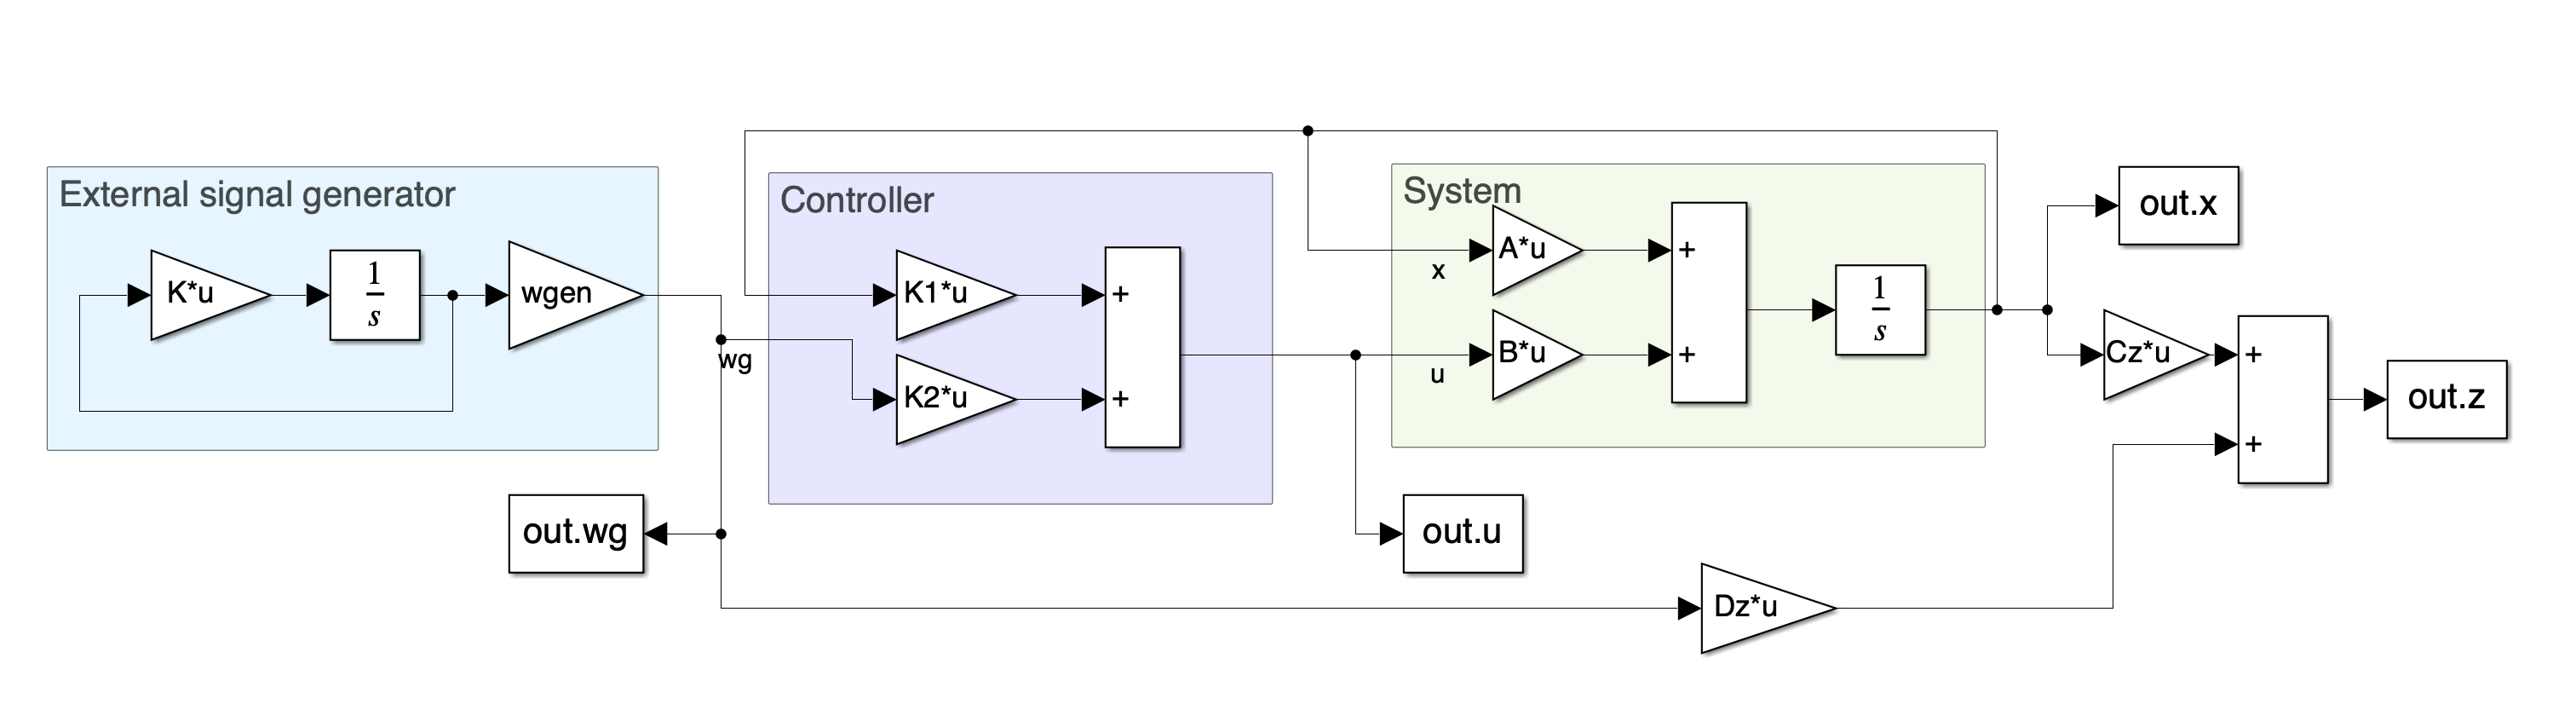
\includegraphics[width=\textwidth]{"media/scheme2.png"}
    \caption{Схема моделирования системы}
    \label{fig:task2_scheme}
\end{figure}
% Для начала возьмем $T = 0.73 \approx \sqrt{3} - 1$. Таким образом, согласно теоретическим расчетам, система будет устойчива.
% должна быть близка к границе устойчивости. Промоделируем (см рис. \ref{fig:task2_out}).
% \begin{figure}[ht!]
%     \centering
%     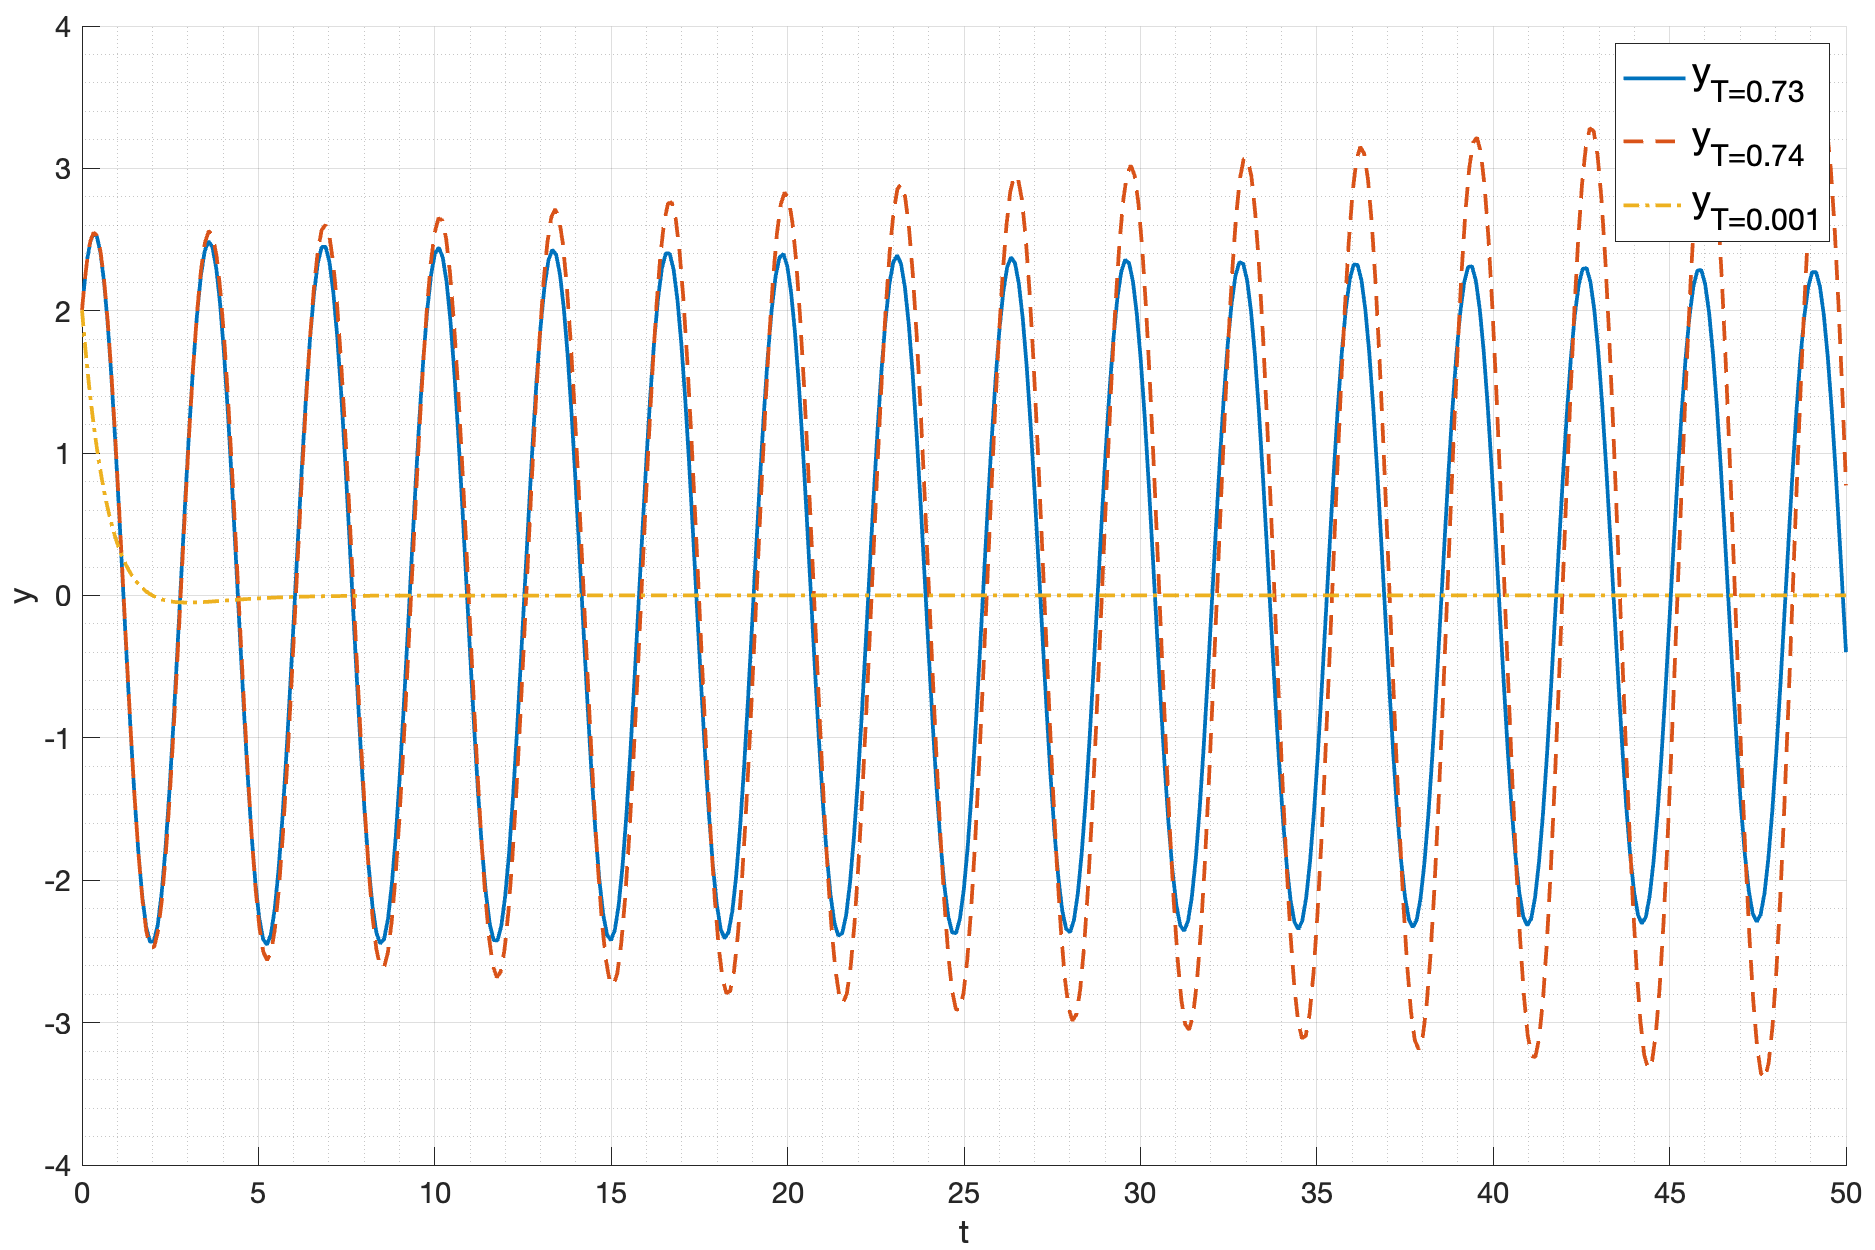
\includegraphics[width=\textwidth]{"media/plots/task2_out.png"}
%     \caption{Свободное движение системы ($T = 0.73$)}
%     \label{fig:task2_out}
% \end{figure}
% Теоретические ожидания подтвердились. Система близка к границе устойчивости, но все еще является устойчивой, 
% так как было выбрана значение несколько меньшее, чем $\sqrt{3} - 1$. Теперь выберем значение $T = 0.74$ и промоделируем систему (см. рис. \ref{fig:task2_out2}).
% \begin{figure}[ht!]
%     \centering
%     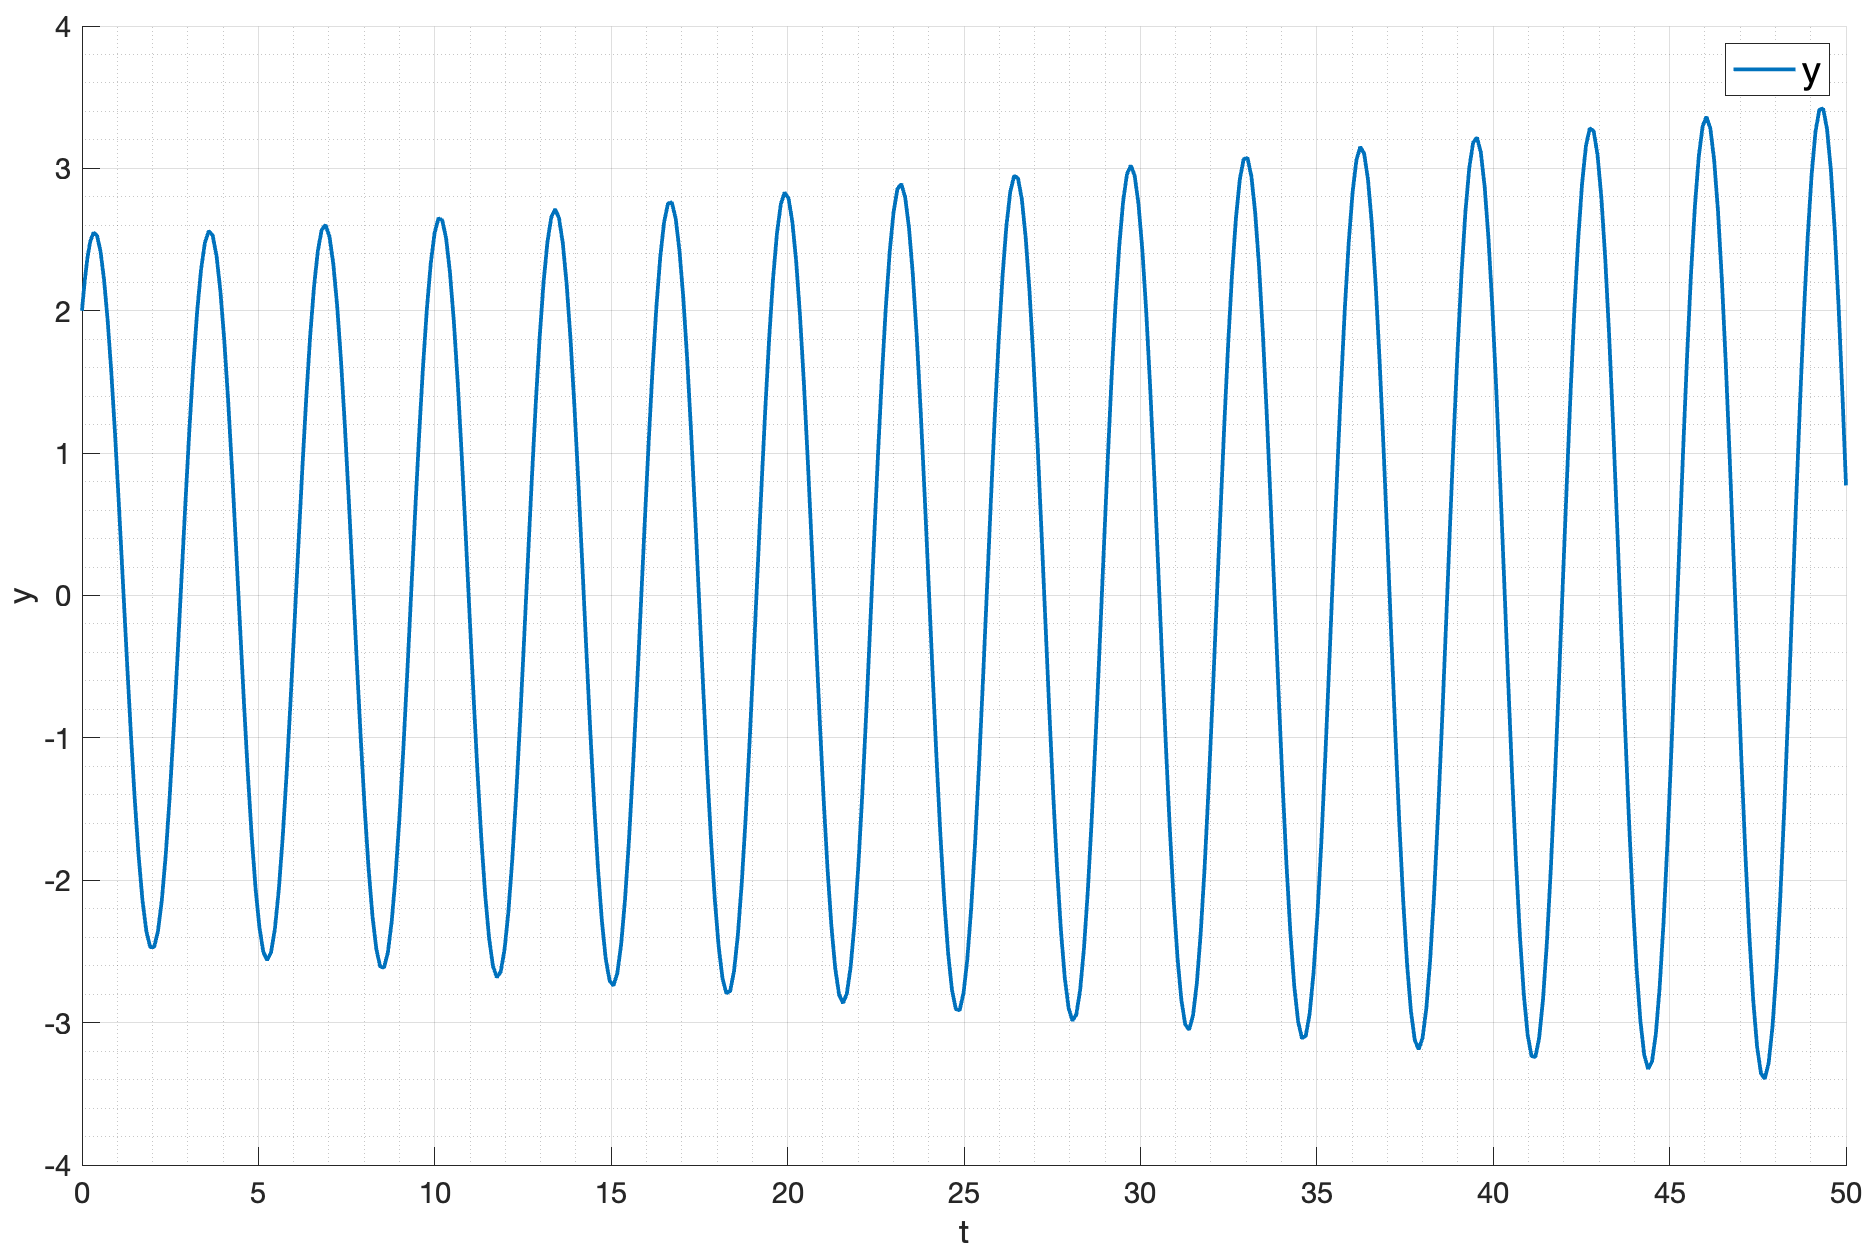
\includegraphics[width=\textwidth]{"media/plots/task2_out2.png"}
%     \caption{Свободное движение системы ($T = 0.74$)}
%     \label{fig:task2_out2}
% \end{figure}
% Теперь видно, что система стала неустойчивой, что подтверждает теоретические расчеты.

% Выберем меньшее значение $T = 0.001$ и промоделируем систему (см. рис. \ref{fig:task2_out3}).
% \begin{figure}[ht!]
%     \centering
%     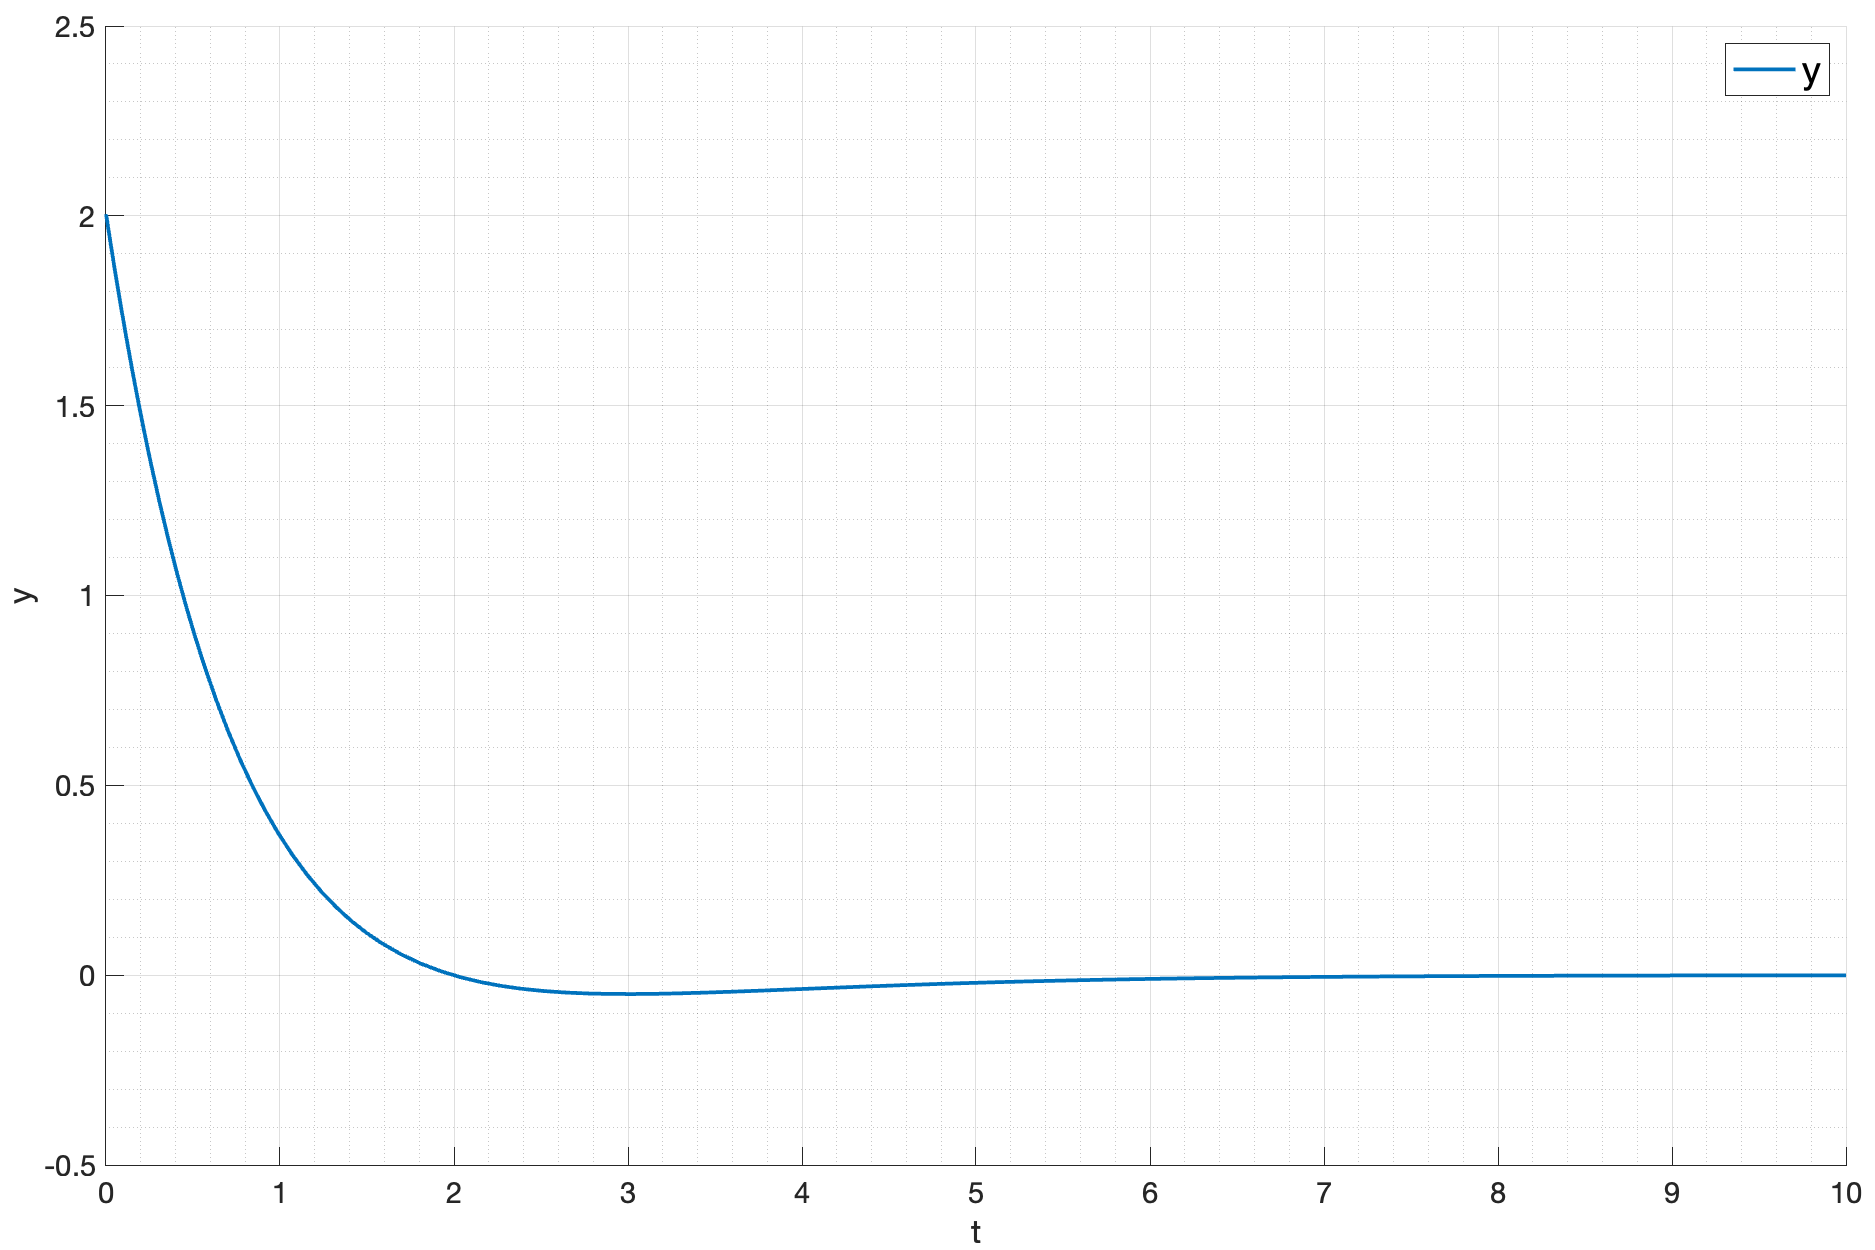
\includegraphics[width=\textwidth]{"media/plots/task2_out3.png"}
%     \caption{Свободное движение системы ($T = 0.001$)}
%     \label{fig:task2_out3}
% \end{figure}

Выберем значения $T = \{0.73, 0.74, 0.001\}$. В первом случае система будет устойчива и близка к границе устойчивости,
во втором случае система будет неустойчива, а в третьем случае система будет устойчива, но менее колебательна.
Результаты моделирования приведены на рис. \ref{fig:task2_out}, \ref{fig:task2_err}.
\begin{figure}[ht!]
    \centering
    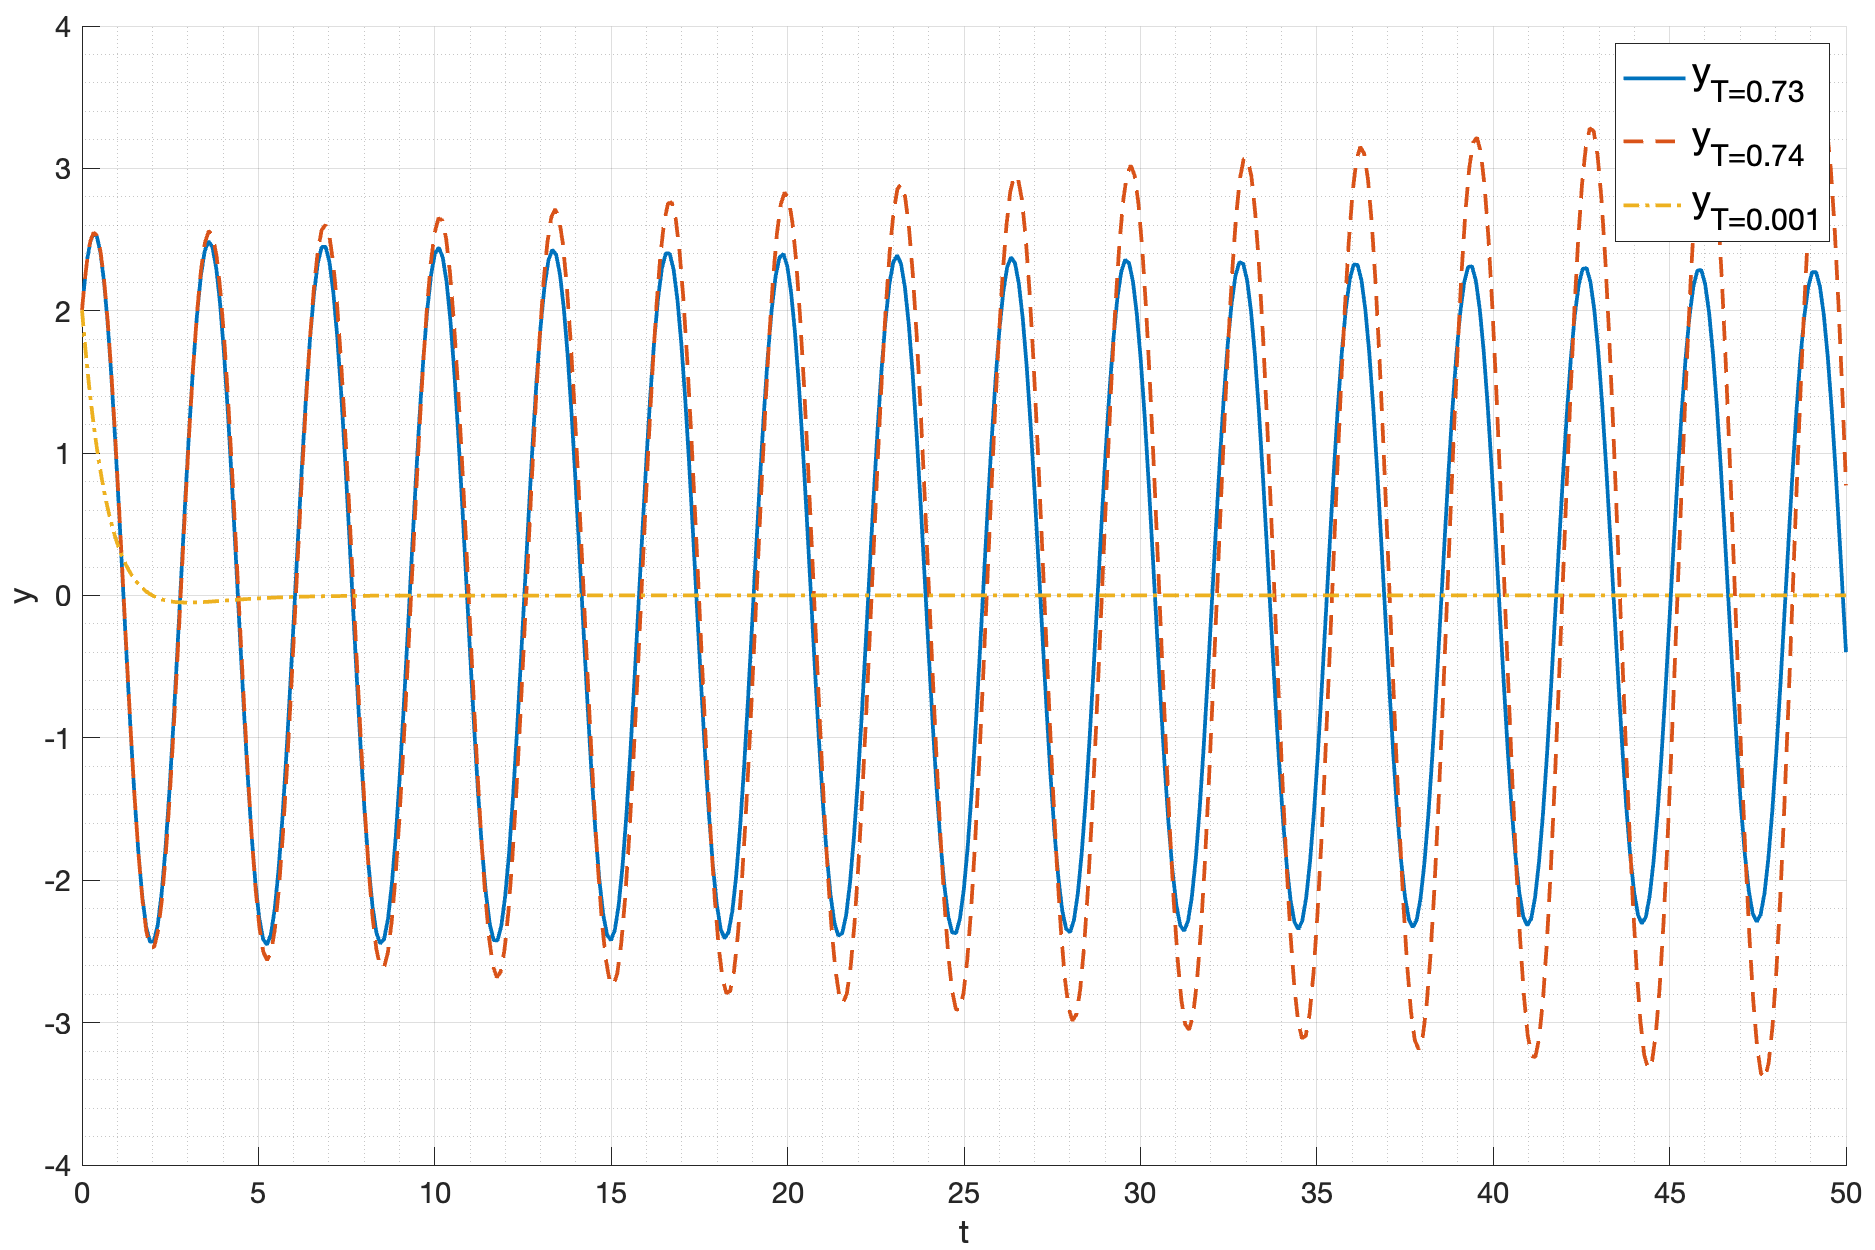
\includegraphics[width=\textwidth]{media/plots/task2_out.png}
    \caption{Графики выходного сигнала}
    \label{fig:task2_out}
\end{figure}

\begin{figure}
    \centering
    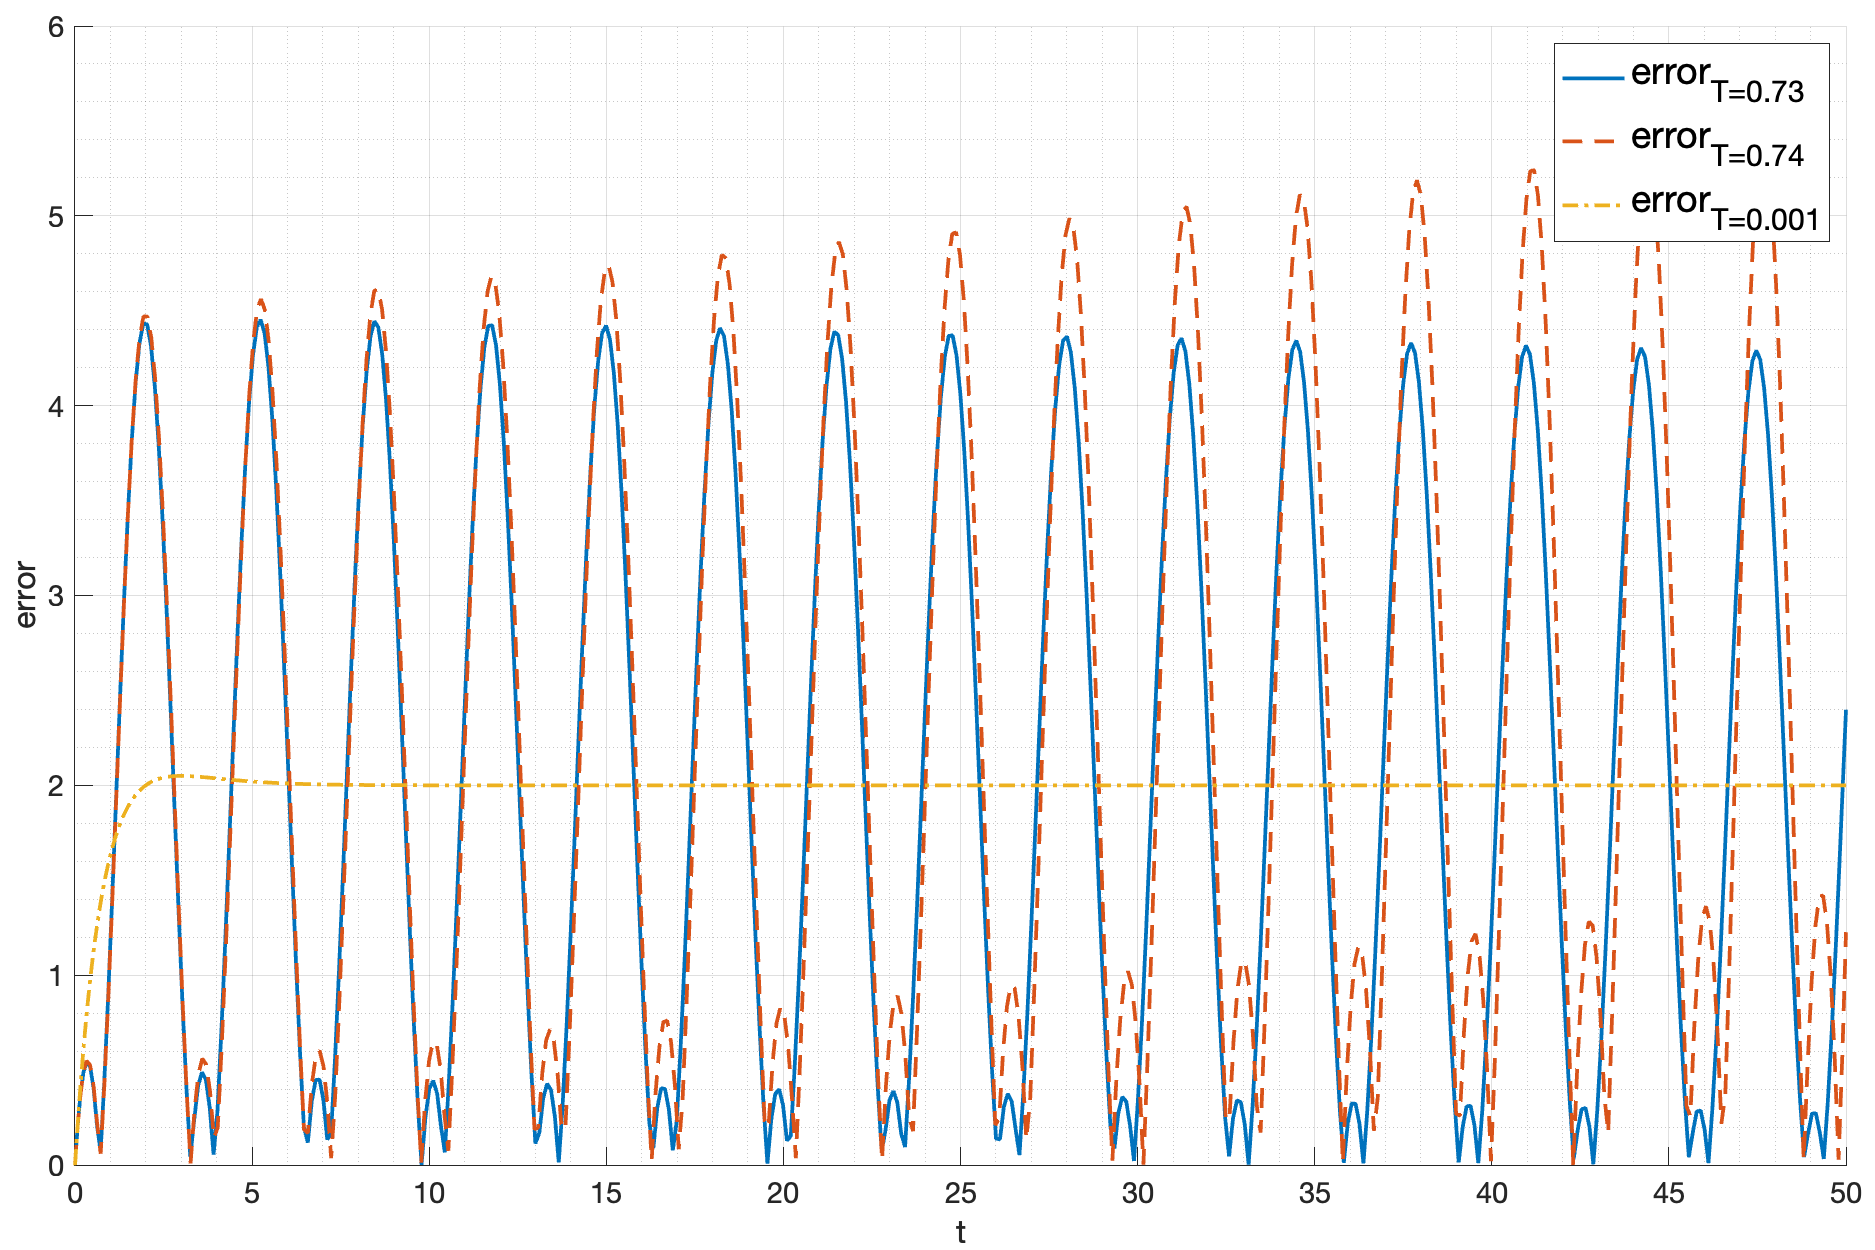
\includegraphics[width=\textwidth]{media/plots/task2_error.png}
    \caption{Графики ошибки}
    \label{fig:task2_err}
\end{figure}


\subsection{Вывод}
В данном разделе было проведено моделирование системы с реальным дифференцирующим звеном. 
Система оказалась устойчивой при $T \in (0, \sqrt{3} - 1)$, что подтверждает теоретические расчеты. 
При уменьшении значения $T$ система становится менее колебательной, так как передаточна 
функция дифференцирующего звена приближается к идеальному дифференцирующему звену. 